\documentclass[a4paper,11pt]{article}

\usepackage[utf8]{inputenc} \usepackage[T1]{fontenc}
\usepackage{fancyhdr} \usepackage{graphicx,subfig} \usepackage{lastpage}
\usepackage{amssymb,amsmath} \usepackage{siunitx} \usepackage[nodayofweek]{datetime}
\usepackage[top=3.5cm,bottom=2.5cm,left=3cm,right=3cm,headheight=40pt]{geometry}
\usepackage{parskip} \usepackage{float} \usepackage{enumitem} \pagestyle{fancy}
\usepackage[colorlinks=true,allcolors=blue]{hyperref} \hypersetup{
	pdfauthor={Michaël Defferrard},
	pdftitle={Project stage 1: Terrain generation},
	pdfsubject={Introduction to Computer Graphics}
}

\lhead{Introduction to Computer Graphics\\Project stage 1: Terrain generation\\Group 19}
\chead{\hspace{2.5cm}EPFL\\\hspace{2.5cm}\shortdate\today\\\hspace{2.5cm}\thepage/\pageref{LastPage}}
\rhead{Michaël \textsc{Defferrard}\\Pierre \textsc{Fechting}\\Vu Hiep \textsc{Doan}}
\cfoot{}

\begin{document}


\section{Overview}



\section{Implementation}

\subsection{Triangle grid}

The vertices and indices arrays are computed by the \texttt{triangle\_grid} function. The sole parameter is the number $N$ of points on the grid. Figures~\ref{triangle_grid_8}, \ref{triangle_grid_16} and~\ref{triangle_grid_64} show the result for different values of $N$. These results were generated by code state at commit \texttt{e63a2600093a1639b25c93ad43a221634e10d892}.

\begin{figure}[ht]
	\centering
	\subfloat[\textsf{GL\_LINE\_STRIP} with $N=8$]{
		\label{triangle_grid_8}
		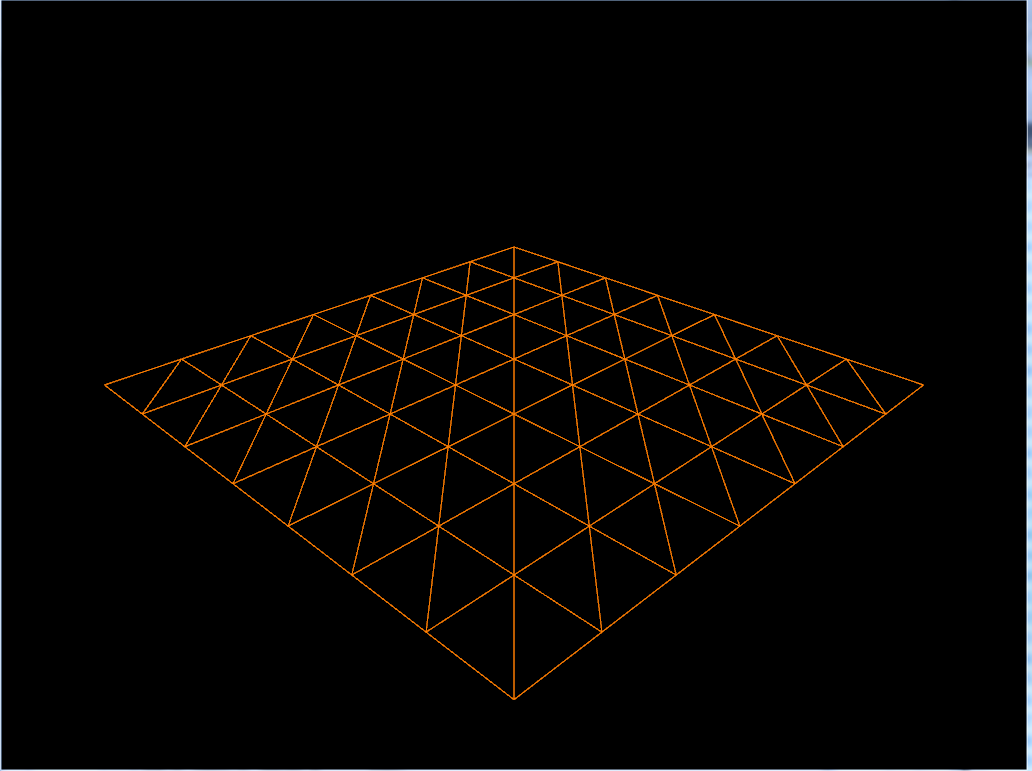
\includegraphics[height=4cm]{{{img_stage1/triangle_grid_8}}}
	} \quad
	\subfloat[\textsf{GL\_LINE\_STRIP} with $N=16$]{
		\label{triangle_grid_16}
		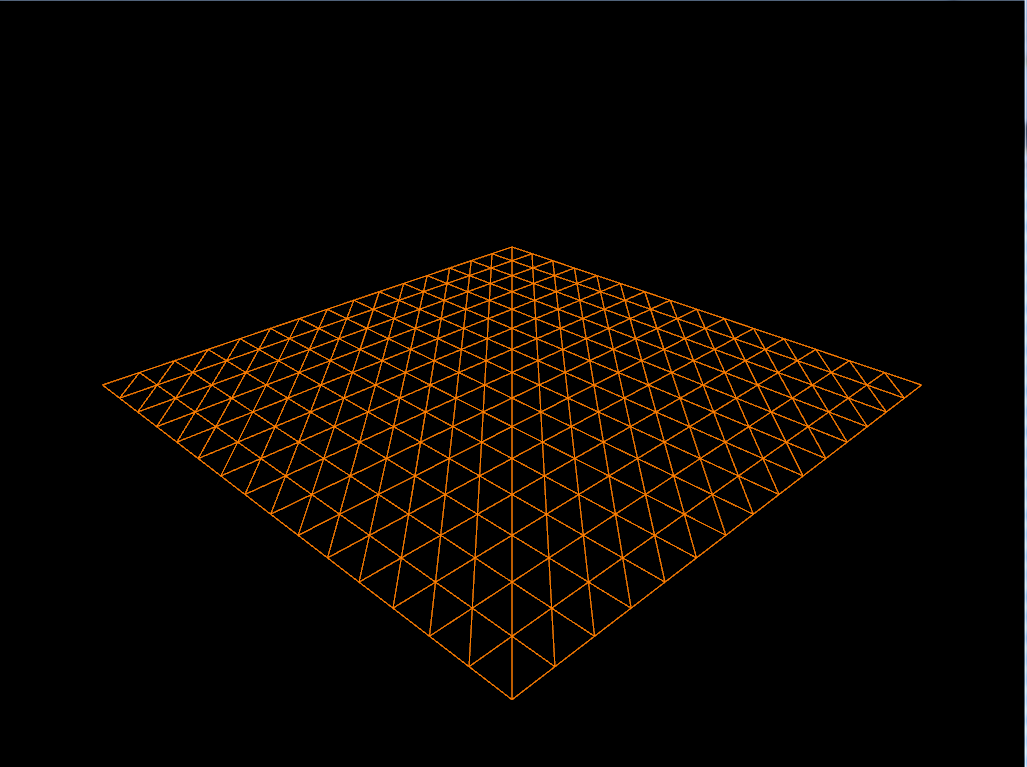
\includegraphics[height=4cm]{{{img_stage1/triangle_grid_16}}}
	} \quad
	\subfloat[\textsf{GL\_LINE\_STRIP} with $N=64$]{
		\label{triangle_grid_64}
		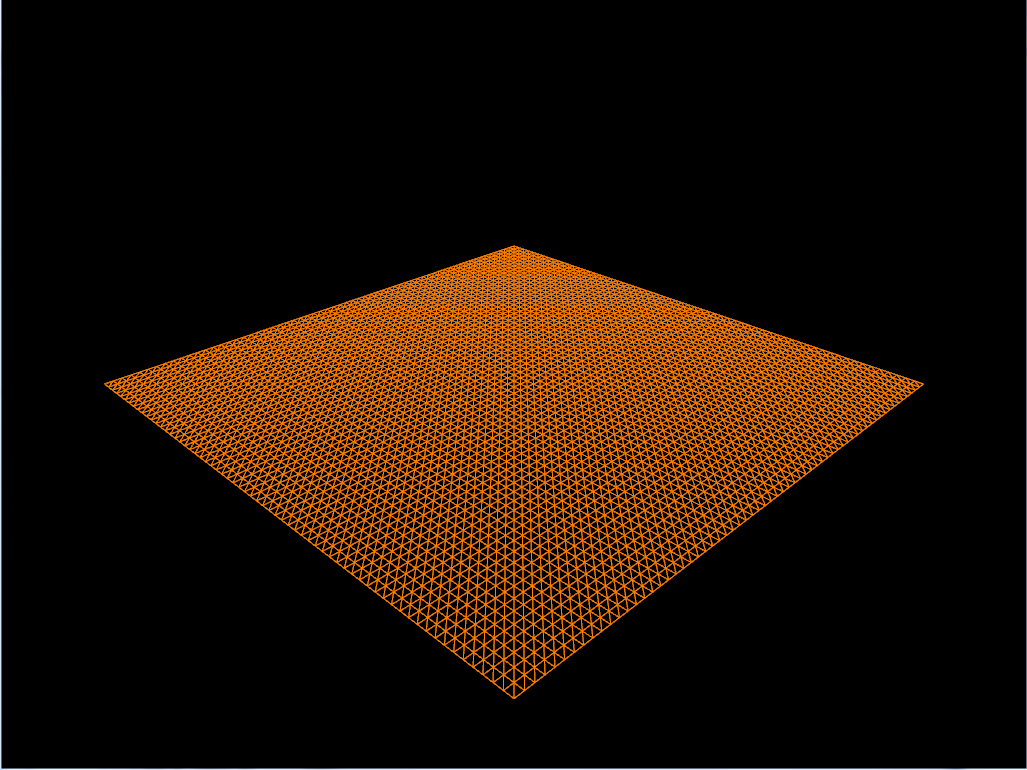
\includegraphics[height=4cm]{{{img_stage1/triangle_grid_64}}}
	} \quad
	\subfloat[\textsf{GL\_TRIANGLES}]{
		\label{triangle_grid_full}
		
\includegraphics[height=4cm]{{{img_stage1/triangle_grid_full}}}
	}
	\caption{Triangle grid}
	\label{triangle_grid}
\end{figure}

When looking at these figures, it seems that a row of triangles is missing, as the outer-line is missing (fig.~\ref{triangle_grid_8}, \ref{triangle_grid_16} and~\ref{triangle_grid_64}). By looking at the generated triangles (fig.~\ref{triangle_grid_full}), it is however clear that this is not the case (all the triangles are drawn). The generation of the first triangle (fig.~\ref{triangle_artifact}) shows it even more clearly.

\begin{figure}[ht]
	\centering
	\subfloat[\textsf{GL\_LINE\_STRIP}]{
		
\includegraphics[height=4cm]{{{img_stage1/triangle_artifact}}}
	} \quad
	\subfloat[\textsf{GL\_TRIANGLES}]{
		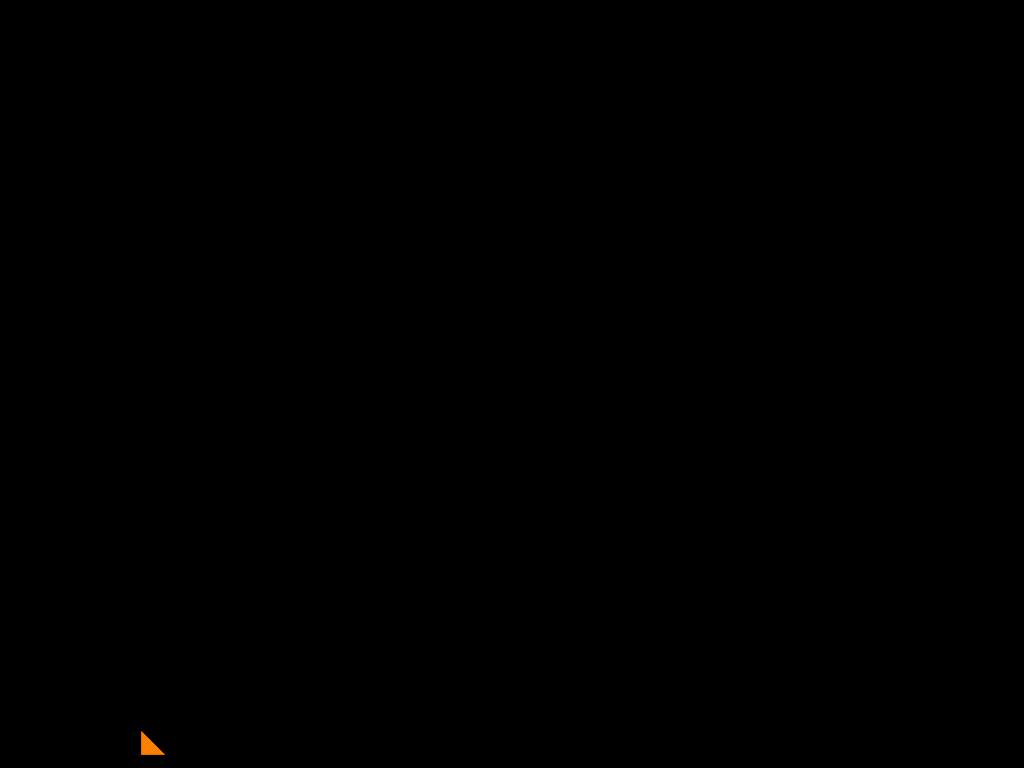
\includegraphics[height=4cm]{{{img_stage1/triangle_artifact_full}}}
	} 
	\caption{First triangle only}
	\label{triangle_artifact}
\end{figure}




\section{Results}



\end{document}
